\section{Analysis of the Experimental Results}
\label{sec:liquid:analysis}

\subsection{Analysis of the Quantum Oscillations}
In a strong magnetic field perpendicular to the sample surface, the Dirac surface electrons are quantized into Landau levels (LLs) with quantum numbers $N = 0,1,\cdots$. Here we take the same definition of the index field $B_n$ as in Ref. \cite{Xiong2012b}, which is also the same as our previous chapters. Thus $B_n$ is the field at which $E_F$ falls between two LLs. This definition can also be naturally extended to the quantum Hall regime.
For Schr\"odinger states, the integer $n$ counts the number of 
occupied LLs (the highest filled LL has $N_{max} = n-1$ with the energy $E = (N_{max}+\frac12)\hbar \omega$, where $\omega$ is the cyclotron frequency). Using the level 
degeneracy $Be/h$ per spin, we then have $1/B_n = ne/(hn_s)$ 
($n_s$ is the surface density, $e$ the elemental charge and $h$ is Planck's constant). Thus the Landau index plot in Schr\"odinger case has a zero intercept.

The Dirac electrons have an extra $\frac12$ shift in their LLs as we have
$n+\frac12$ filled LLs when $B = B_n$ (now $N_{max} = n$).
The additional $\frac12$ derives from the $N=0$ LL due to the particle-hole symmetry, or equivalently, 
from the $\pi$-Berry phase intrinsic to each Dirac cone~\cite{Kim}. 
The relation between $1/B_n$ and $n$ is now 
$ 1/B_n = (n+\frac12)(e/h n_s)$ -- a straight line that 
intercepts the $n$-axis at $n = -\frac12$. 
As we discussed in previous chapters, $G_{xx}$ provides a reliable way to decide $B_n$ even when the bulk conductance contributes significantly. And it is a local minimum at $B_n$ for both Dirac and Schr\"odinger electrons. Therefore, we can leverage the difference in the intercepts to distinguish the Dirac electrons and the Schr\"odinger ones.

\begin{figure}[!htbp]
  \begin{center}
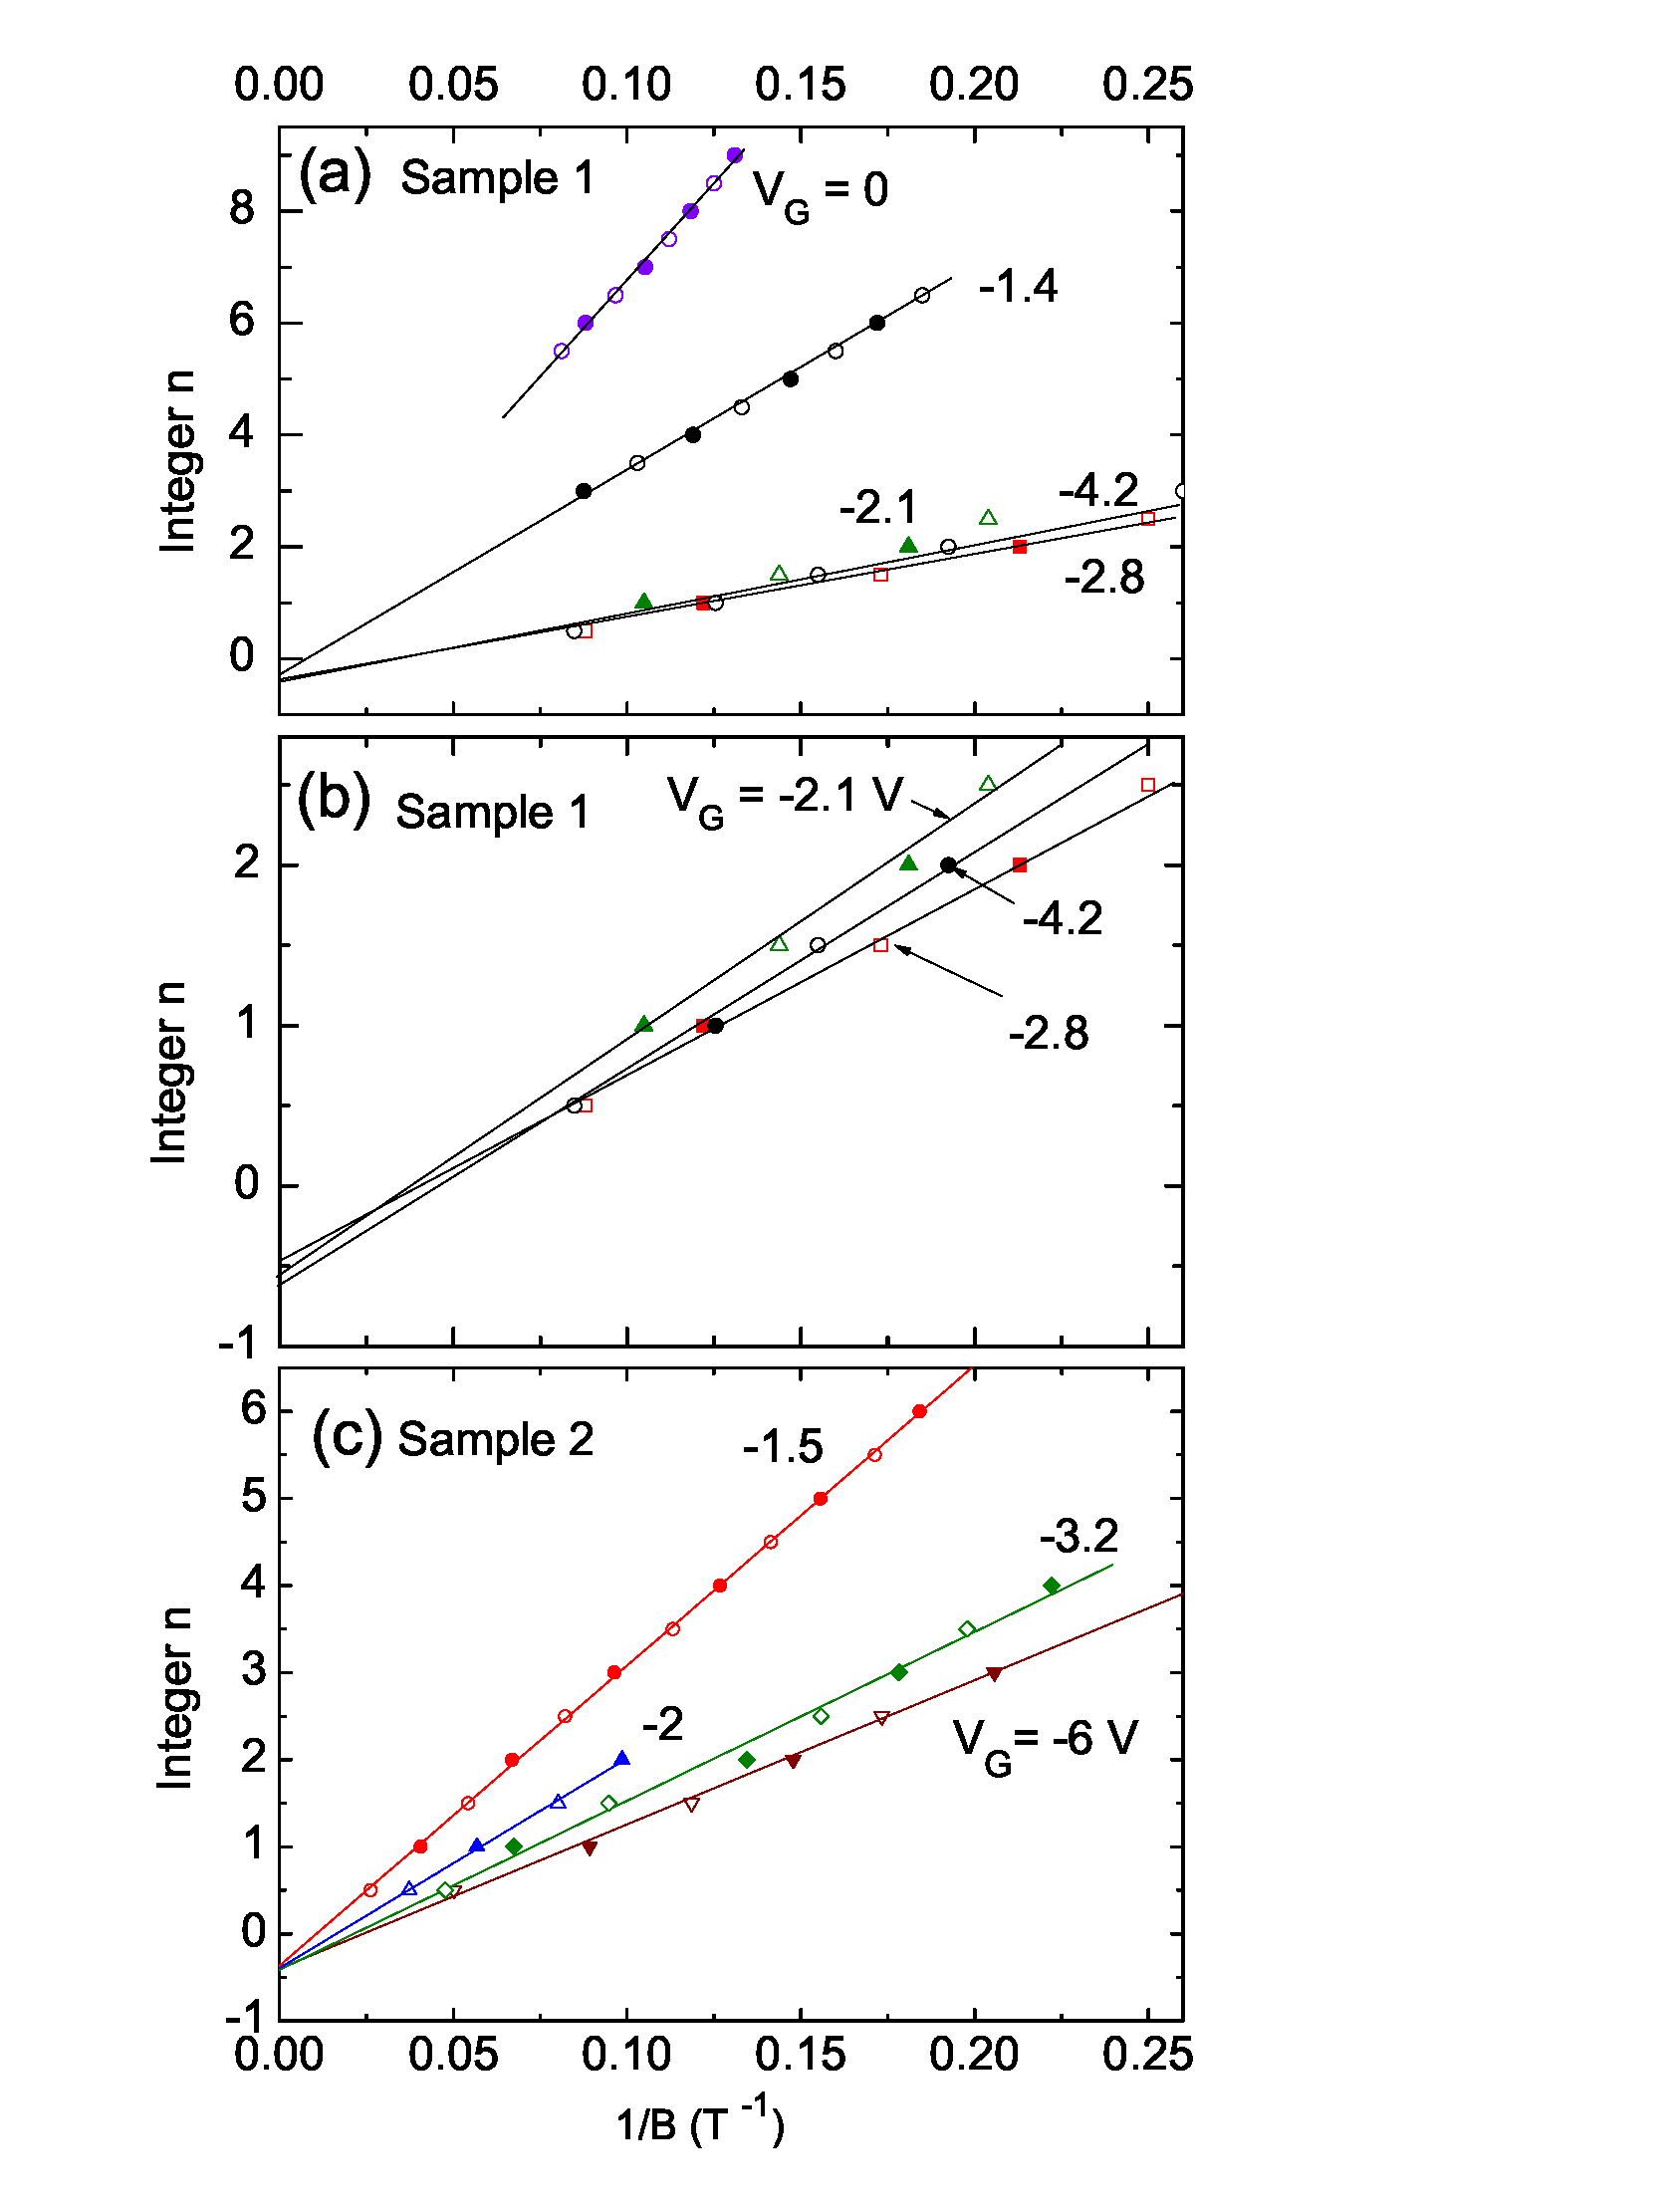
\includegraphics[width=0.85\linewidth]{ch-liquid/figures/FigIndexAll}
\caption{\label{figIndex} 
Index plots of the integer $n$ vs. $1/B_n$ at selected $V_G$ in Sample 1 (Panels a and b) and 2 (Panel c).
Maxima of $\Delta\rho_{xx}$ (solid symbols), corresponding to the index fields $B_n$, are plotted against $n$. Minima (open symbols)
are plotted against $n+\frac12$.
Panel (a): As $V_G$ changes from 0 to -2.1 V, the slope of the best fit lines decreases by six times, indicating a decrease of the carrier density by six times as well. Further increase
in $|V_G|$ leads to saturation of the slope. In Panel (b), the high-bias curves are displayed in expanded vertical scale to determine the intercept. In the limit $1/B\to 0$, the best-fit lines have intercepts at -0.46, -0.56 and -0.61 respectively for different $V_G$. They are close to $\frac12$ (mod 1), consistent with a Dirac dispersion.
The intercepts for Sample 2 (Panel c) also cluster near -0.45 in the limit $1/B\to 0$.
}
  \end{center}
\end{figure} 


However, if the resistivity curves are used to determine the Landau indices, $B_n$ should be identified with the \emph{maxima} in $\Delta\rho_{xx}$ as we discussed in the previous chapter. This is useful when the Hall data are not available. From the $\Delta\rho_{xx}$ v.s. $1/B$ curves in Fig. \ref{figSdH_Vg}, we plot as solid symbols $B_n$ in Sample 1 against the integers $n$ in Fig. \ref{figIndex}a
(the open symbols corresponding to the minima are plotted against $n+\frac12$). The straight lines in the figure are the least square fit to the index plots. The slopes of the fitted straight lines yield the Fermi surface area $S_F$ at different $V_G$. 
As $|V_G|$ increases from 0 to 2.8 V, the slopes of the best-fit lines 
decrease by a factor of 6.4, reflecting a steep decrease in $S_F$. 
This decrease saturates when $|V_G|$ exceeds 2.1 V. Such a decreasing $S_F$ at negative $V_G$ is expected as the anions on the sample surface deplete the $n$-type surface states.  

Then we leverage the intercepts of the fit lines to investigate the Dirac nature of the surface states at different $V_G$. As discussed in previous chapters, sometimes the slope of the index plot changes from the low field regime to the high field part. And the intercepts are fixed by the high field indices. Therefore, we show the high-field behavior for $|V_G|>$ 2.1 V in expanded scale in Panel (b) to obtain a higher accuracy in determining the intercepts. At various large bias values, the intercepts all gather around $n = -\frac12$ 
(-0.46, -0.56 and -0.61) for Sample 1. 

In the Landau index plot for Sample 2 (Panel c), we find that $S_F$ decreases by a factor
of 2 between $V_G$ = -1.4 and -6 V. In the limit $1/B\to 0$, the intercepts are at
$n= -0.35$, -0.40 and -0.42.  These values are all significantly closer to $-\frac12$ than 0 or 1.
The lowest index we obtain at the highest $B$ in both samples is $n_{min}=\frac12$, indicating that $E_F$ lies in the middle of the broadened $N=1$ Dirac LL. As we argued in the previous chapter, such a small $n_{min}$ is important for us to reduce the uncertainties and rigorously exclude an intercept at $n=0$ in the limit $1/B\to 0$. We illustrate the uncertainties incurred in Fig. \ref{figIndexError}a. At $V_G$=0 V, where the LL index is high, the uncertainties $\delta B_n$ in determining the index fields are typically $\pm5\%$ (circles). As shown, it could lead to a considerable spread in the allowed intercepts as we extrapolate the fitted line to the n-axis (the lowest datum corresponds to n = 5.5). By comparison, at the gate voltage $V_G$ = -2.8 V 
(squares), the lowest index is n = 1. This significantly shrinks the spread in the allowed intercepts. The same advantage may be achieved by applying an intense $\bf B$ up to 45 T, as done in Ref. \cite{Xiong2012b}.
Therefore, by showing the $-\frac12$ intercepts at different $V_G$, we have provided more conclusive evidence for the Dirac and surface nature of the SdH oscillations on top of our previous discussions.

\begin{figure}[!htbp]
  \begin{center}
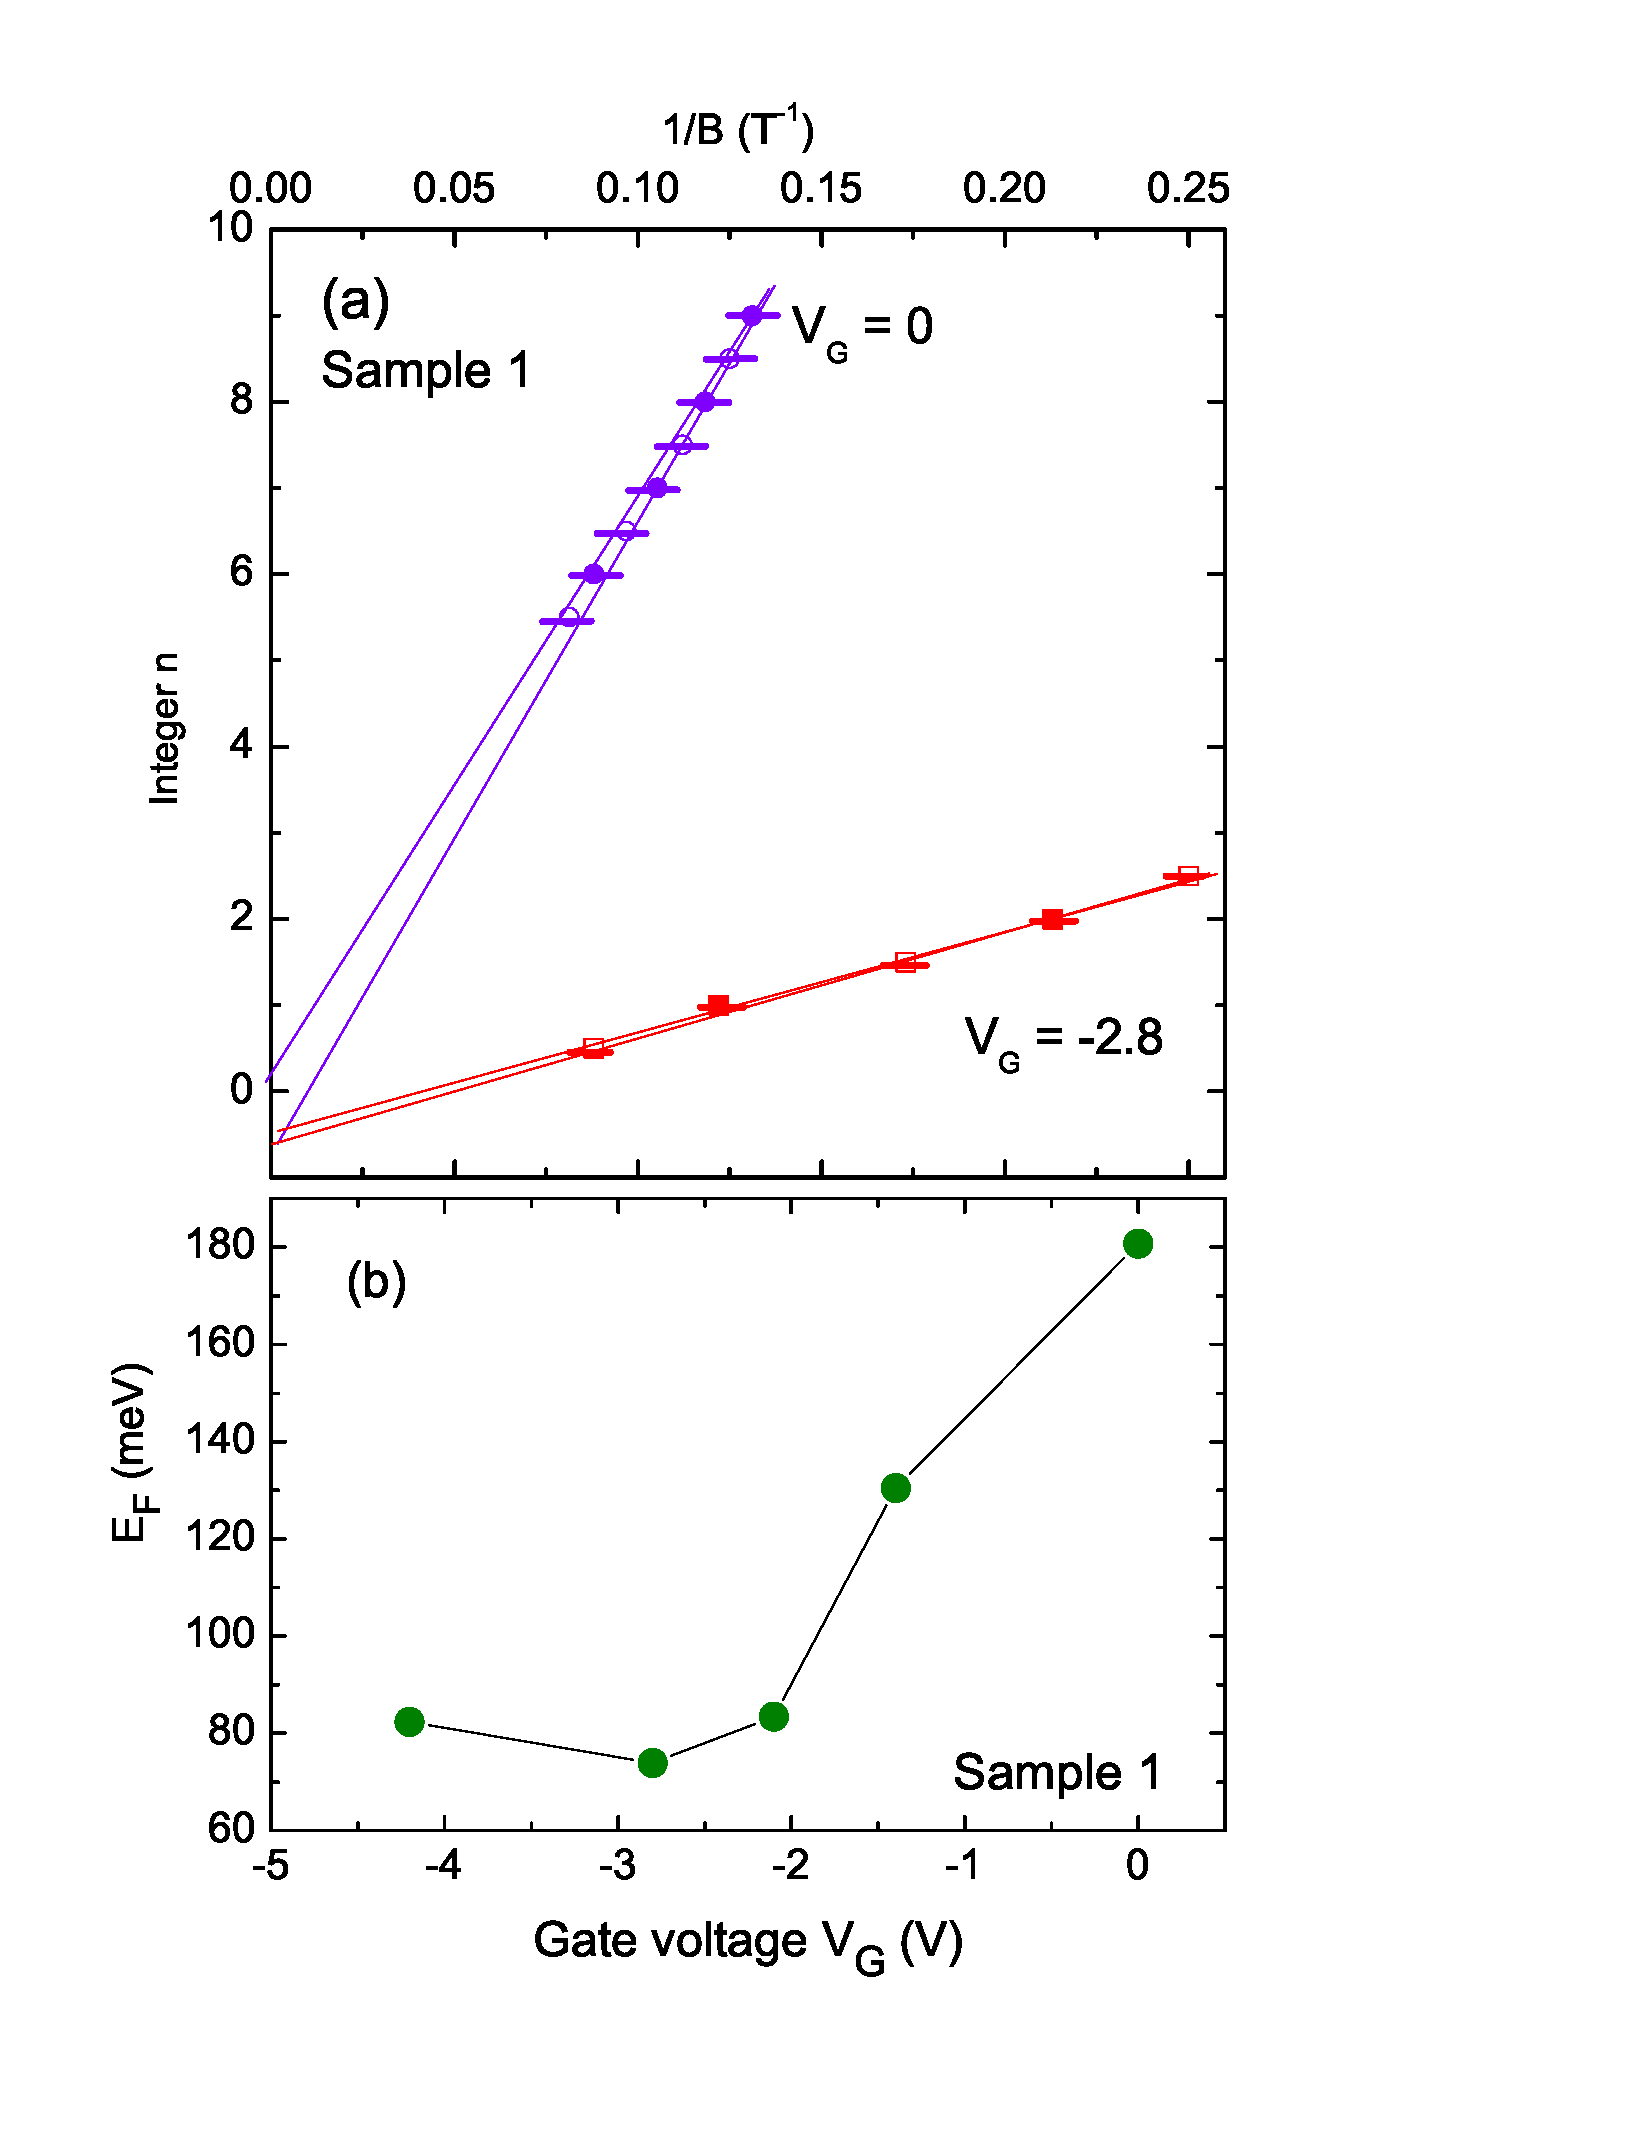
\includegraphics[width=0.85\linewidth]{ch-liquid/figures/FigIndexError.eps}
\caption{\label{figIndexError} 
Comparisons of extrapolations of the index plot to the limit $1/B \to 0$ for index fields measured with $V_G$ = 0 (circles) and measured with $V_G$ = -2.8 V (squares) in sample 1. (b) Variation of $E_F$ with applied $V_G$ in sample 1 ($E_F$ is measured from the Dirac point). The FS cross-section $S_F$ is converted to $E_F$ by $E_F = \hbar v\sqrt{S_F/\pi}$ 
using $v$ = 6$\times 10^5$ m/s~\cite{Xiong2012}. For $|V_G|> 2 V$, the decrease in $E_F$ saturates.
} 
  \end{center}
\end{figure} 


We also calculated the Fermi energy by $E_F=\hbar v \sqrt{S_F/ \pi}$ at different $V_G$, where $S_F$ is inferred from the slopes of the index plots in Figs. \ref{figIndex}. The Fermi velocity we use here is $v_F = 6 * 10^5 m/s$~\cite{Xiong2012}. Fig. \ref{figIndexError}(b) shows that $E_F$ in Sample 1 has been dramatically reduced from 180 meV to around 80 meV when $V_G$ changes from 0 V to -2 V. Thereafter, it remains at $\sim80$ emV. We also use this information below to estimate the depletion capacitance. Another thing we notice is that $E_F$ stops decreasing when $|V_G|$ exceeds 2 V, possibly due to the saturation of the anion layer and the incoming chemical reactions at large $|V_G|$. It also shows the limitation of the gating power by ionic liquid. Besides, since the Dirac point in Bi$_2$Te$_2$Se is close to the top of the valence band, we have not induced any band inversion in this experiment (otherwise we would have an accumulation layer of holes).

To obtain further information of the surface states at different $V_G$, we fit the SdH oscillations to the Lifshitz-Kosevich expressions (shown as dashed curves) as displayed in Fig. \ref{figSdH_Vg}. The field dependence of the oscillation amplitudes yields the surface mobility $\mu_s$. As shown in Fig. \ref{figHall}b, the surface mobility improves from 720 cm$^2$/(Vs) at 0 V to 2,480 cm$^2$/(Vs) at -4.2 V. Fig. \ref{figHall}c shows that the surface density $n_s = k_F^2/(4\pi)$ (per surface) decreased by approximately 4 times until it saturates at $V_G$ = -2.1 V. We suspect that this saturation at large $|V_G|$ is due to either the chemical reactions or the possibility that $E_F$ starts to touch the top of the valence band.

Another important number that characterizes the quality of TI crystals is the conductance ratio between the surface and the bulk $\eta \equiv G^s/G^b$ in zero $B$ (with $G^r \equiv G^r_{xx}(0)$, $r=s,b$). Such ratio describes the portion of the current that flows on the surface of a TI, and can be used to compare different TI materials and devices. It is also of great practical value to improve this $\eta_H$. In our Sample 1, $\eta\sim 0.05$ is quite small (compared with $\eta\sim 1$ obtained in Ref.~\cite{Xiong2012}). However, we notice that the Hall conductance ratio $\eta_H = G^s_{xy}/G^b_{xy}$ which is between the surface and bulk Hall conductance, is enhanced by $\mu_s/\mu_b$ on top of $\eta$ in the Drude model. Since the surface and bulk mobility ratio $\mu_s/\mu_b$ is large in our samples, $\eta_H$ could also be large. 



\subsection{Analysis with a Two-Band Model}

In light of this conjecture, we fit the measured Hall conductivity by a two-band Drude semiclassical model. In the fitting, we fix the surface mobility $\mu_s$ and density $n_s$ with the ones inferred from quantum oscillations. Since the bulk mobility is low, the bulk term only relies on one parameter, i.e.  $n_b\mu_b^2$. Therefore, we only need to tune one parameter to obtain the best-fit curve in the two-band model. This strategy greatly reduces any possibility of overfitting which is typical in a two-band model with multiple parameters. Thus, it can give us reliable results about the bulk properties. The fitting formula we use for $\sigma_{xy}$ is:
\be
\sigma_{xy}= n_se\mu_s\frac{\mu_sB}{t[1+ (\mu_s B)^2]} + n_be\mu_b^2 B,
\label{eq:sxy}
\ee
where the first term is $G^s_{xy}/t$, with $t$ the thickness (50 $\mu$m in Sample 1). 
As $n_s$ and $\mu_s$ are fixed by analysis of the SdH oscillations, the surface term is 
non-adjustable. The second term is the bulk Hall conductivity
$\sigma^b_{xy}$ in the low-mobility limit. We show the fitting results in Fig. \ref{figHall}a and compare it with the field dependence of $\sigma_{xy}$ in the data.
With the sole adjustable parameter $P_b\equiv n_b\mu_b^2$, we find that Eq. \ref{eq:sxy} 
(dashed curves) fits the experimental results very well at multiple $V_G$.
To emphasize the surface contribution, we have also plotted $G^s_{xy}/t$ as inner and faint solid curves in Fig. \ref{figHall}a. 
Combining $P_b$ with the zero-$B$ value of
$\sigma^b_{xx}$, we finally separate and obtain $n_b$ and $\mu_b$ for each value of $V_G$.
We report their values at different $V_G$ in Figs. \ref{figHall}b and \ref{figHall}c. 
The small values of $\mu_b$ (20-30 cm$^2$/Vs) result in a 
large $\mu_s/\mu_b\sim$ 100 and $\eta_H\sim$ 5. We notice that the large $\mu_s$ could also explain the weak-field curvature of $\sigma_{xy}$ in Fig. \ref{figHall}a as the large $\mu_s$ yields a resonance peak at low fields. Also, since the resonance peak generated by $\mu_s$ grows as $\mu_s$ becomes larger, it may also account for the curvature enhancement in $\sigma_{xy}$ with an increasing $|V_G|$.

\begin{figure}[!htbp]
  \begin{center}
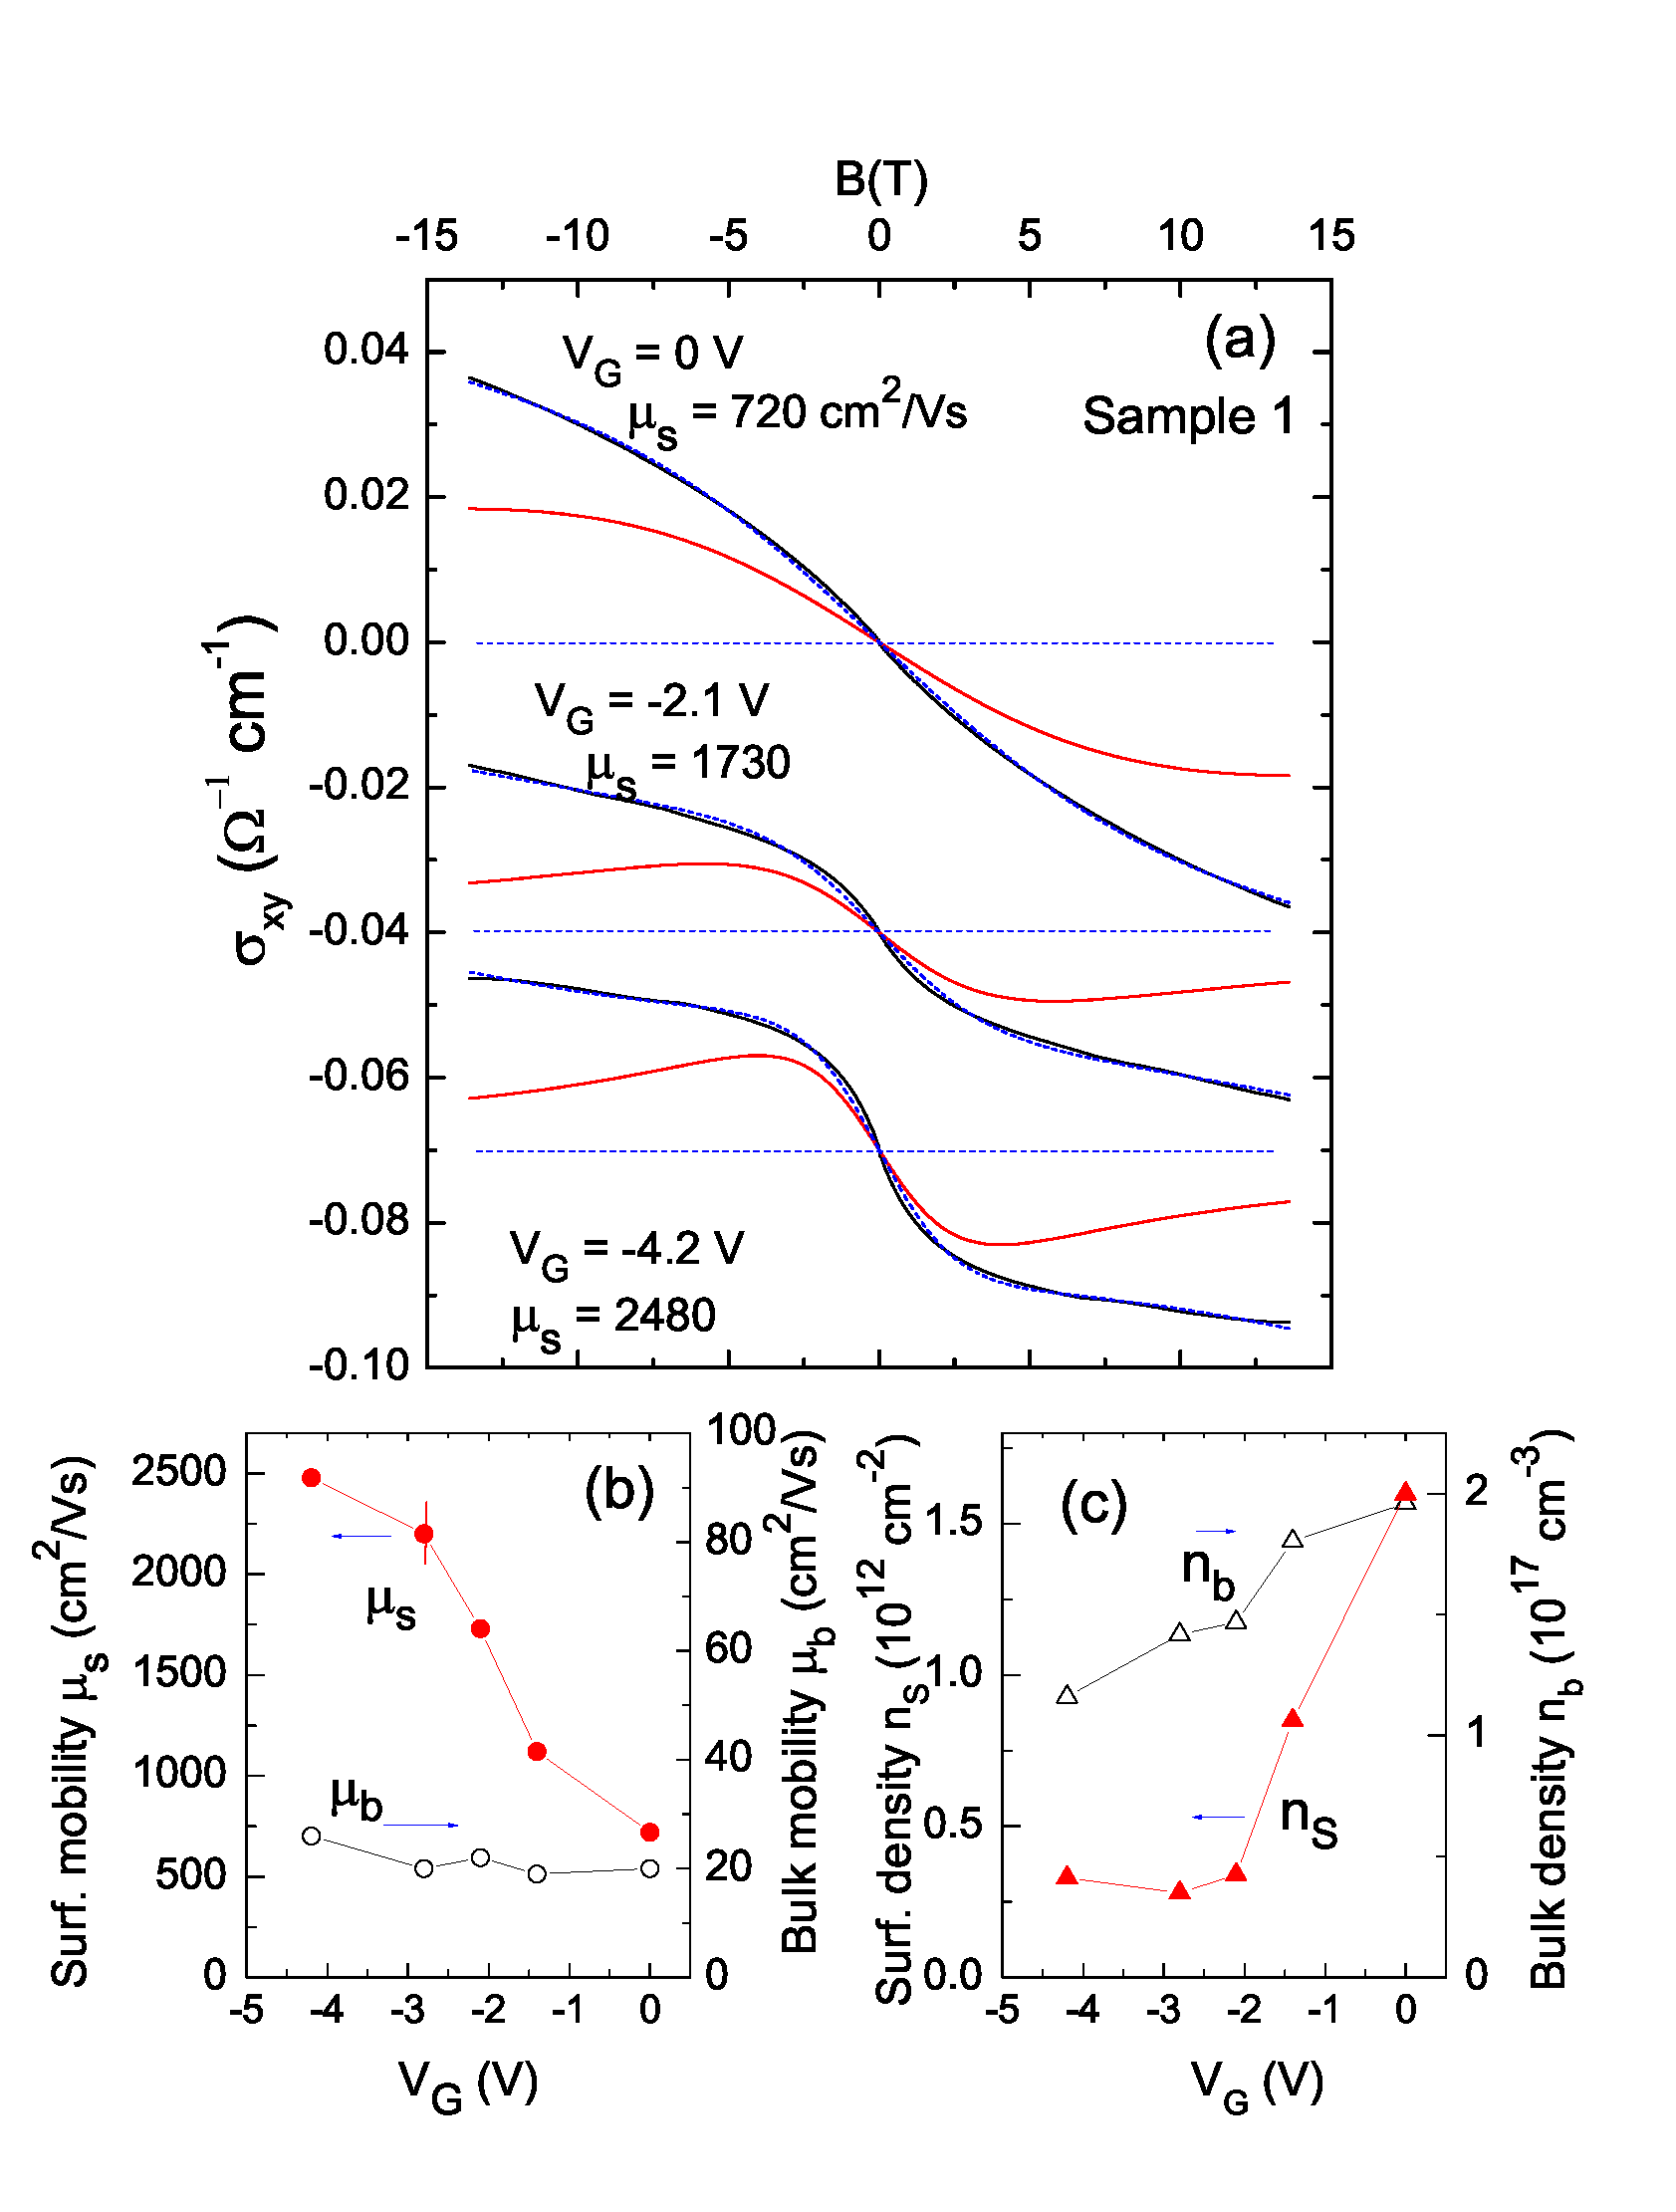
\includegraphics[width=0.85\linewidth]{ch-liquid/figures/FigHallMob3}
\caption{\label{figHall} (color online) 
Panel (a): The observed Hall conductivity $\sigma_{xy}$ vs. $B$ in Sample 1,
showing weak-$B$ curvatures at 3 values of $V_G$
(curves displaced for clarity). At each $V_G$, the outer curves are the 
data (solid black curve) and the fit to Eq. \ref{eq:sxy} (superposed blue dashed curve). The inner
(red, solid) curve is the surface term
$G^s_{xy}/t$ fixed by $n_s$ and $\mu_s$. (Weak SdH oscillations are apparent in the
observed $\sigma_{xy}$.) The difference 
between the outer and inner curves is the bulk term $\sigma^b_{xy}$. 
At $V_G$ = -4.2 V, $G^s_{xy}/t$ accounts for 83$\%$ of
$\sigma_{xy}$ in weak $B$. 
Panel (b) shows that, with increased gating, $\mu_s$ increases from 720 to 2,480 cm$^2$/Vs 
while $\mu_b$ stays very small (20-30 cm$^2$/Vs). Panel (c) 
compares the sharp decrease in $n_s$ with the mild change in $n_b$ with gating. When $|V_G|$ is larger than
2 V, $n_s$ saturates.
}
  \end{center}
\end{figure} 


The above analysis indicates the coexistence of high-mobility surface Dirac electrons and a larger population of bulk electrons in our Bi$_2$Te$_2$Se samples. Because of the 100-fold difference in mobilities,
the Dirac surface electrons account for 83$\%$ of the total weak-$B$ Hall conductance at large $|V_G|$. Since we only includes one surface in calculating the surface Hall conductance, and it already accounts for the majority of the total $\sigma_{xy}$. There is no room left for a comparably large $G^s_{xy}$ for the other surface. With the parameters above, we estimate that the Hall contribution from the other surface 
is less than 2$\%$ of $\sigma_{xy}$. It also implies a low mobility on the other surface ($\mu_s$ is $<$300 cm$^2$/Vs), which explains why we do not resolve the other surface in SdH oscillations.





%The large enhancement of $\mu_s$ (Fig. \ref{figHall}b)
%by the liquid gating method is perhaps the most intriguing 
%feature reported here. To our knowledge, this is the first realization of 
%enhancement of surface SdH amplitudes by an \emph{in situ} technique.%~\cite{mobility}
%A recent STM experiment~\cite{Beidenkopf2011} reveals that
%the Dirac Point closely follows spatial fluctuations of the local
%potential on length scales of 30-50 nm. This could lead to strong scattering
%of surface electrons. We speculate that, under liquid gating, the anions accumulate
%at local maxima in the potential, thereby levelling out the strongest spatial fluctuations.%~\cite{scatter}
%The results provide encouragement that alternative routes that even out local
%potential fluctuations can lead to further improvements in $\mu_s$.


\subsection{Depletion-layer Capacitance, Screening and Impurity Band}

Besides the information about the surface states, the above gating experiments can also provide us with quantitative results on the electronic parameters in the bulk depletion region. This is important because it yields detailed properties of the bulk and can guide future gating experiments. In particular, an advantage of our experiment is that the SdH oscillations fix both $n_s$ and $E_F$ of the surface carriers (hence the surface electrostatic potential $\varphi(0)$) at each applied $V_G$. Then we can combine it with the carrier density and conductivity of the bulk carriers, as well as the anion charge $Q$ accumulated on the crystal surface, to depict a detailed picture of the band-bending model and perform self-consistency checks in the depletion capacitance. We follow the standard analysis of field-effect gating as introduced in Ref.\cite{SternRMP,Ashcroft,Sze}. We also provide more details in the appendix. 

%Our main results are on the tuning of the SdH oscillations of the Dirac surface states. However, the 
%experiment also yields quantitative results on the electronic parameters in the depletion region,
%which provide detailed picture of what happens under liquid gating.
%A useful feature of the experiment is that, at each value of the applied gate voltage $V_G$, we can measure via the SdH oscillations
%both $n_s$ and $E_F$ of the surface carriers
%(hence the surface electrostatic potential $\varphi(0)$). In addition, we measure
%the carrier density and conductivity of the bulk carriers, and the anion charge $Q$ accumulated on the
%crystals surface. The 5 quantities provide a detailed picture of the
%band-bending process as well as self-consistency checks in determining the depletion capacitance. 
%We apply the standard analysis of field-effect gating~\cite{SternRMP,Ashcroft,Sze},
%which is summarized in Appendix \ref{appcap}. 

When the chemical potential lies inside the band gap at $V_G$=0 V, as in the case of Bi$_2$Te$_2$Se, the gating effect will induce band bending. Instead, if $E_F$ is high in the conduction band (as the case in as-grown Bi$_2$Se$_3$), the applied $\bf E$
leads to Thomas Fermi screening~\cite{Ashcroft} for which the screening length is
$\lambda_{TF} = \sqrt{\pi a_B/4k_F}$ is typically a few $\rm \AA$ ($a_B = \hbar^2/me^2$ is the Bohr radius).
For a hard gap (impurity band absent), a negative $V_G$ leads to a depletion region.
However, despite displaying a very large
bulk resistivity (2-6 $\Omega$cm) at 4 K, the current generation of Bi$_2$Te$_2$Se crystals still have a substantial
bulk carrier density ($n_b\sim$ 2$\times 10^{17}$ cm$^{-3}$). This implies an impurity band that extends across the gap.
Nonetheless, band bending over a significant depletion region ($\sim$10 $\mu$m) is observed.
We will analyze this situation at the end of this section after we estimate the depletion capacitance.


For $V_G < 0$ V, the electric field $\bf E$ from the anions repels bulk electrons away from the surface,
exposing the ionized donors within the depletion width $d$. 
Figure \ref{figGate}a shows a sketch of the band bending near the surface exposed to the liquid.
For finite $V_G$, the ionic liquid polarizes to form, in effect, two capacitors each with
spacing of the order of the molecular radius $a$. Each capacitor stores the charge $Q$. 
The capacitor at the gate electrode 
has an area $A'$ much larger than that of the capacitor at the crystal surface $A$, so that
most of the potential drop $V_G-V_s$ falls across the latter ($V_s$ is the voltage 
corresponding to $\varphi(0)$ and the ground is taken deep in the bulk at $x\to +\infty$).
In Sample 1, $A$ = 2.9 mm$^2$ and $A'$ = 30 mm$^2$. 
The $E$-field produced by the anion layer just to the left of the crystal surface is 
$E(0^-) = Q/A\epsilon_0$.


%%%%%%%%%%%%%%%%%%%%%%%%%%%%%%%%%%
%%%%%%%%%%%%%%%%%%%%%%%%%%%%%%%%%%
%%%%%%%%%%%%%%%%%%%%%%%%%%%%%%%%%% FIGURE 7
\begin{figure}[!htbp]
  \begin{center}
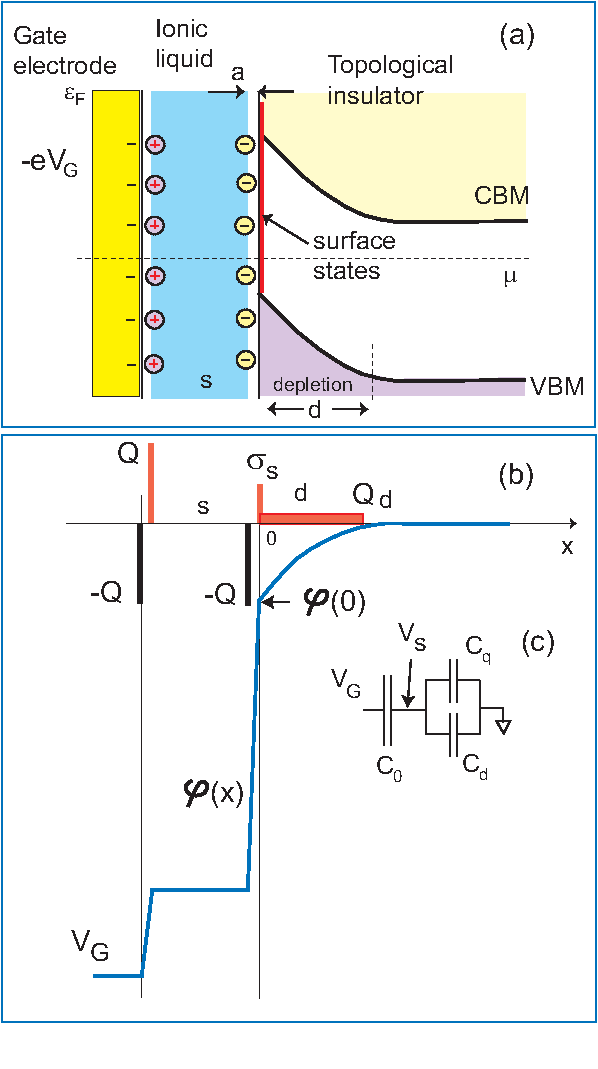
\includegraphics[width=0.65\linewidth]{ch-liquid/figures/FigGate.pdf}
\caption{\label{figGate} 
Sketch of band bending and the profiles of $\rho(x)$ and $\varphi(x)$ in the liquid gating experiment.
Panel (a) shows upwards bending of the bands induced by a negative gate voltage $V_G$. The cations and anions 
define two serial capacitors with spacing $a$ (molecular radius). The depletion layer in the bulk of the TI extends
a distance $d$. Panel (b) displays the charge distribution versus $x$. The negative charge $-Q$ on the gate electrode is
replicated by the anion layer separated by $a$ from the TI surface. This is compensated by the sum of the surface charge density
$\sigma_s$ and the ionized impurity charges inside the depletion layer. The electric potential $\varphi(x)$ corresponding to
$\rho(x)$ is sketched. Panel (c) shows the circuit of the equivalent capacitors $C_0$, $C_d$ and $C_q$.
}
  \end{center}
\end{figure} 



In Fig. \ref{figGate}b, we sketch the profiles of the charge density $\rho(x)$ and the 
electrostatic potential $\varphi(x)$ (the $x$-axis is normal to the surface). 
Within the liquid, $\rho(x)$ of the cations and anions are taken to 
be delta functions of strength $\pm Q$. In the TI, the surface charge density is represented by
a delta function ($\sigma_s$). Within the bulk, however, $\rho(x)$ is distributed 
over the depletion layer to a depth $d$. As a guide, it is convenient to adopt the usual approximation, 
whereby $\rho(x)$ is taken to be uniform for $0<x<d$. 
In the uniform-charge approximation, $\varphi(x)$ varies as $-(x-d)^2$ in the depletion region.
Its value at the surface is then
\be
\varphi(0) = -N_ded^2/(2\epsilon_0\epsilon_s),
\label{phi0}
\ee
where $N_d$ is the donor impurity concentration and $\epsilon_s$ the screening dielectric parameter.
The charge $Q_d$ induced in the depletion width by $\varphi(0)$ defines the depletion capacitance
$C_d = N_dedA/\varphi(0) = \epsilon_0\epsilon_s A/d$. The surface charge density $\sigma_s$ 
induced by $\varphi(0)$ is represented by the quantum capacitance
$C_q = \sigma_s/\varphi(0) = e^2(dn_s/d\mu)$. Clearly, $C_d$ and $C_q$ are in parallel
combination (Fig. \ref{figGate}c).

The large slope change at $x=0$ mainly reflects the strong dielectric screening in the bulk of the
TI ($\sigma_s$ makes a negligible contribution). Thus the intense $E$-field produced by the
anions is strongly screened by polarization effects inside the crystal ($E(0^-)\gg E(0^+)$). 
As shown in Fig. \ref{figGate}c, the parallel combination of $C_d$ and $C_q$ is in 
series with $C_0$, the series combination of the cation and anion capacitances.
In all samples, we find that $C_d\gg C_q$, so we may ignore the quantum capacitance in the discussion below.

%\noindent
%\emph{Magnitude of $C_d$}\\
As shown in Fig. \ref{figIndexError}b, $E_F$ in Sample 1 decreases by $\sim$100 mV when the applied $V_G$ is -2 V.
Thus, only a small fraction ($\sim 1/20$) of the applied gate voltage is effective in bending the band ($V_s$ = -0.1 V).
We can use this observation to determine the depletion capacitance $C_d$.
The value of $C_0/A$ for ionic liquids is 11-12 $\mu$F/cm$^2$~\cite{Koch}.
(From the expression, $C_0/A = \epsilon_0\epsilon_{liq}/a$, this corresponds to $\epsilon_{liq}$ = 4, and $a$ = 3 $\rm\AA$.) 
Using the ratio $V_s/(V_G-V_s)\sim C_0/C_d$ (neglecting $C_q$), we estimate that $C_d/A\simeq$ 240 $\mu$F/cm$^2$.

Alternatively, we may estimate $C_d$ by integrating the ionic current to find the charge $Q$.
For Sample 1 with $V_G$ = -2 V, the ionic charge current deposits a total negative ionic charge at the surface equal to
$-Q/A\sim 2\times 10^{14}e$/cm$^2$ = -3.2$\times 10^{-5}$ C/cm$^2$. 
Since $Q/A$ is stored in $C_d$ by the voltage $V_s\sim$ 0.1 V,
we have $C_d/A\sim$ 320 $\mu$F/cm$^2$, which is 33$\%$ larger than the first estimate, but within our uncertainties.
The main source of uncertainty is the actual area coated by the anions. Because the ions can coat the silver paint
contacts and voltage and current leads, the area can exceeds that of the crystal $A$ by 50 to 100$\%$.

Using $\frac Q A = N_d e d + \sigma_s$, we may estimate the depletion width $d$ as a check.
The donor density $N_d$ is roughly equal to the bulk density observed at 4 K, $n_b~\sim 2\times 10^{17}$ cm$^{-3}$.
This gives $d\simeq$ 10 $\mu$m. The deep penetration of the depletion region into the bulk
is consistent (within a factor of 2) with the 40$\%$ change observed in the resistivity and Hall coefficient at 4 K.

Taking the range $C_d/A$ = 240-320 $\mu$F/cm$^2$, we find that 
the depletion capacitance is 5,000-6,000$\times$ larger
than the values commonly observed in a Si-MOSFET device ($C_{d,Si}/A\simeq$ 0.05-0.06 $\mu$F/cm$^2$~\cite{SternRMP,Sze}).
The enhancement points to a very large polarizability in the ground state of Bi$_2$Te$_2$Se
when $E_F$ lies inside the energy gap. This is perhaps unsurprising given that the 
energy gap in high-purity Si is devoid of impurity states. By contrast, 
Bi$_2$Te$_2$Se at 4 K displays a small, but metallic conductivity arising from a large population of impurity-band electrons.


Here, we resume discussion of the finite DOS in the gap.
To create an extended depletion region with significant band bending, as we have here (Fig. \ref{figGate}a), 
the weak bulk conductivity must be further driven to zero throughout the depletion region
in order to sustain a finite $E$-field (otherwise one has Thomas-Fermi screening with the very short screening length 
$\lambda_{TF} \simeq$ 6 $\rm\AA$
for $n_b$ = 2$\times 10^{17}$ cm$^{-3}$m). To explain how band-bending is sustained over a large depletion region,
we need the existence of a mobility edge in the 
impurity band. Throughout the depletion layer, $E_F$ lies below the mobility edge so that the
conductivity is vanishingly small at 4 K. Because impurity-band states close to the mobility edge 
have a greatly enhanced polarizability in an $E$-field, we expect the electronic contribution to 
dielectric constant $\epsilon_s$ to be orders of magnitude larger than the lattice contribution.
Measurements of $C_d/A$ probe directly the electronic polarizability in the depletion region. A
possible scenario is described in the appendix.

